%AUTOR: KAMIL ŁANGOWSKI 
%EMAIL: kamil.langowski@gmail.com
\documentclass[a4paper]{article}

\usepackage{polski}
\usepackage{amsfonts}
\usepackage{listings}
\usepackage{graphicx}
\usepackage{tikz}
\usepackage{geometry}


\lstdefinestyle{mystyle}{
    basicstyle=\ttfamily\footnotesize,
    breakatwhitespace=false,         
    breaklines=true,                 
    captionpos=b,                    
    keepspaces=true,                 
    numbers=left,                    
    numbersep=5pt,                  
    showspaces=false,                
    showstringspaces=false,
    showtabs=false,                  
    tabsize=2
}

\lstset{style=mystyle}

\title{Regresja logistyczna}
\author{Kamil Łangowski \\ Wydział Fizyki Technicznej i Matematyki Stosowanej \\ Politechnika Gdańska}
\begin{document}
\maketitle
\newpage
\section{Teoria}
\subsection{Wstęp}
W tej sekcji omówimy model uczenia maszynowego nazywany regresją logistyczną (ang. \textit{logistic regression}). Wbrew swojej nazwie nie jest to problem regresji, lecz klasyczny problem klasyfikacji. Nazwa "regresja logistyczna" jest, być może, myląca, jednak ze względów historycznych została ugruntowana. Rozważać będziemy problem klasyfikacji binarnej, to znaczy taki, w którym zmienna objaśniana może należeć tylko do dwóch klas. 
\subsection{Prosta regresja logistyczna}
Załóżmy, że $Y$ jest zmienną objaśnianą o charakterze dyskretnym (jakościowym). Przykładowo niech $Y$ na podstawie uzyskanych danych na temat wykrytego nowotworu określa, czy jest on złośliwy. Jeżeli tak, to $Y=1$, jeżeli nie, to $Y=0$. Regresja logistyczna, w odróżnieniu od regresji liniowej, nie stara się przewidzieć zmiennej $Y$ na podstawie zmiennej objaśniającej $X$ bezpośrednio, a określa prawdopodobieństwo, że $Y$ będzie przyjmować wartość jednej z możliwych kategorii. Niech $X= \{x_i\}_{i=1}^n$ będzie zmienną objaśniającą, która w naszym przykładzie zawiera dane uzyskane na temat nowotworu; powiedzmy, że $X$ reprezentuje jego wielkość. Wówczas definiujemy prawdopodobieństwo warunkowe
\begin{equation}
    Pr(Y = 1|x_i),
\end{equation}
które określa, prawdopodobieństwo złośliwości nowotworu na podstawie jego rozmiaru. Innymi słowy wyraża prawdopodobieństwo przynależności obserwacji $x_i$ do klasy $Y=1$. W skrócie zapisywać będziemy $P(x_i)$, gdzie
\begin{equation}\label{(2.23)}
    P(x_i) = Pr(Y=1|x_i).
\end{equation}
Podobnie jak w przypadku regresji liniowej, w dalszym ciągu staramy się znaleźć zależność $Y$ od $X$, która będzie liniowa i w najlepszym stopniu oddawać będzie relację wyrażoną w {(2)}. Użycie "standardowej" funkcji liniowej jest niewskazane, ze względu na fakt, iż przyjmuje ona wartości spoza zakresu $[0,1]$, co w kontekście wartości prawdopodobieństwa jest niemożliwe w interpretacji.  Istnieje ciągła funkcja, która osiągając wartość zależną od $x_i$ na przedziale $[0,1]$ pozwala określić przynależność $x_i$ do $Y=1$ lub do $Y=0$. Funkcję tę  nazywamy funkcją logistyczną lub funkcją sigmoidalną. Wyraża się wzorem
\begin{equation}
    P(x_i) = \frac{e^{\beta_0 + \beta_1x_i}}{1 + e^{\beta_0 + \beta_1x_i}},
\end{equation}
równoważnie oznaczamy też przez 
\begin{equation}\label{(2.25)}
    f_{\beta_0,\beta_1}(x_i) = \frac{1}{1 + e^{-(\beta_0 + \beta_1x_i)}}.
\end{equation}
 W przypadku, gdy wartość funkcji jest bliższa $0$ obserwacja $x_i$ zostanie przypisana do $Y=0$, w przeciwnym razie przypisana zostanie do $Y=1$. Funkcja sigmoidalna znajduje zastosowanie także w sztucznej inteligencji, w szczególności w sztucznych sieciach neuronowych.  Na rysunku \ref{r(2.5)} przedstawiono wykres funkcji sigmoidalnej.
\begin{figure}[ht]
    \centering
    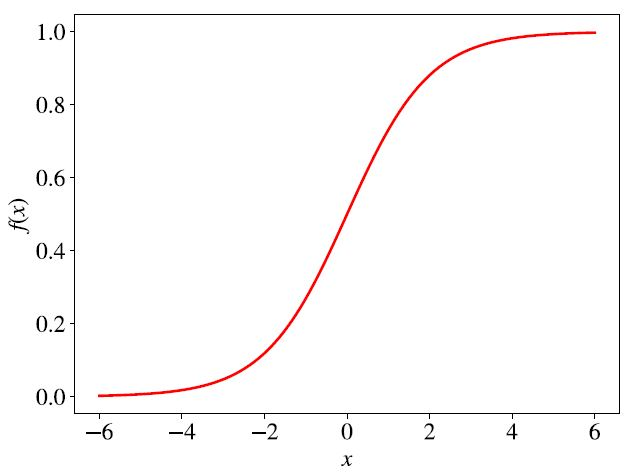
\includegraphics[width=300 pt, height = 200 pt]{SIGMOID_FUNC_HUNDRED.JPG}
    \caption{Wykres funkcji sigmoidalnej.}
    \label{r(2.5)}
\end{figure}

\newpage
\subsection{Określenie wartości parametrów}
Podobnie jak w przypadku regresji liniowej napotykamy problem odpowiedniej estymacji parametrów $\beta_0$ i $\beta_1$. W przypadku regresji logistycznej zamiast używania metody najmniejszych kwadratów posługujemy się metodą szukania maksimów funkcji wiarygodności (ang. \textit{likelihood function}). Załóżmy, że mamy $n$ par obserwacji $\{(x_i, y_i)\}_{i=1}^n$, wtedy funkcja wiarygodności wyraża się wzorem
\begin{equation}\label{(2.26)}
    L(\beta_0, \beta_1) = \prod_{i =  1}^n{\left(f_{\beta_0,\beta_1}(x_i)\right)^{y_i}\left(1-f_{\beta_0,\beta_1}(x_i)\right)^{(1-y_i)}}.
\end{equation}
Wyrażenie $(f_{\beta_0,\beta_1}(x_i))^{y_i}(1-f_{\beta_0,\beta_1}(x_i))^{(1-y_i)}$ oznacza, że jeżeli klasa $i$-tej obserwacji jest równa $1$, to element $(1-f_{\beta_0,\beta_1}(x_i))^{(1-y_i)}$ jest równy jedności, analogicznie dla $y_i = 0$.
W praktyce, z uwagi na wygodę obliczeń,  zdarza się, że używana jest logarytmiczna modyfikacja funkcji {(2.26)}. Funkcja ta wyraża się wzorem
\begin{equation}\label{(2.27)}
    \ln\left(L(\beta_0, \beta_1)\right) = \sum\limits_{i=1}^n{y_i\ln\left(f_{\beta_0,\beta_1}(x_i)\right)+ (1-y_i)\ln\left(1-f_{\beta_0,\beta_1}(x_i)\right)}.
\end{equation}
W odróżnieniu od {(5)} w celu znalezienia optymalnych wartości współczynników $\beta_0$ i $\beta_1$ poszukujemy minimów funkcji {(6)}, jednakże wartości współczynników uzyskane na oba sposoby są identyczne. W przeciwieństwie do regresji liniowej nie istnieje jednoznaczna metoda znajdywania minimów i maksimów powyższych funkcji. Zamiast tego korzysta się z rozwiązań numerycznych takich jak np. metoda spadku gradientu.

\subsection{Wielowymiarowa regresja logistyczna}
Możemy rozważać sytuacje, w których $X = (X^{(1)}, X^{(2)}, \dots , X^{(d)})$. Wówczas funkcja {(2.25)} wyraża się wzorem
\begin{equation}
    f_{\beta_0,\dots,\beta_d}(x_i) = \frac{1}{1 + \exp{\left(-\left(\beta_0 + \sum\limits_{j=1}^d\beta_jx^{(j)}_i\right)\right)}}.
\end{equation}
W tym przypadku również możemy posługiwać się metodą największej wiarygodności w celu ustalenia współczynników $\beta_i$ dla $i = 1,2,\dots, d$.
\newpage


\section{Przykład}
\subsection{Opis zbioru}
Będziemy operować na zbiorze danych \textit{breastcancer} znajdującym się w pakiecie \textit{OneR}. Dane z omawianego zbioru pochodzą ze Szpitala Uniwersyteckiego Uniwersytetu w Wisconsin i dotyczą cech fizycznych nowotworu piersi oraz faktu, czy nowotwór jest złośliwy bądź nie.
\subsection{Cel}
 W niniejszym przykładzie dokonamy predykcję złośliwości nowotworu piersi na podstawie atrybutów, dotyczących cech nowotworu wyrażonych w wartościach całkowitoliczbowych z zakresu $[1,10]$.
\subsection{Kod programu}
Importujemy niezbędne pakiety:
\begin{lstlisting}[language=R, frame=single]
library(OneR)
library(caret)
\end{lstlisting}
Pakiet \textit{OneR} -- zawiera zbiór danych oraz funkcję służącą do ewaluacji modelu klasyfikacji. Wczytujemy zbiór danych oraz wyświetlamy informacje na jego temat:
\begin{lstlisting}[language=R, frame=single]
dane = breastcancer
str(dane)
summary(dane)
\end{lstlisting}
\begin{lstlisting}[language=R, frame=single]
'data.frame':	699 obs. of  10 variables:
 $ Clump Thickness            : int  5 5 3 6 4 8 1 2 2 4 ...
 $ Uniformity of Cell Size    : int  1 4 1 8 1 10 1 1 1 2 ...
 $ Uniformity of Cell Shape   : int  1 4 1 8 1 10 1 2 1 1 ...
 $ Marginal Adhesion          : int  1 5 1 1 3 8 1 1 1 1 ...
 $ Single Epithelial Cell Size: int  2 7 2 3 2 7 2 2 2 2 ...
 $ Bare Nuclei                : int  1 10 2 4 1 10 10 1 1 1 ...
 $ Bland Chromatin            : int  3 3 3 3 3 9 3 3 1 2 ...
 $ Normal Nucleoli            : int  1 2 1 7 1 7 1 1 1 1 ...
 $ Mitoses                    : int  1 1 1 1 1 1 1 1 5 1 ...
 $ Class                      : Factor w/ 2 levels "benign","malignant": 1 1 1 1 1 2 1 1 1
\end{lstlisting}
Zbiór zawiera 699 obserwacji (wierszy) nowotworów i 10 atrybutów (kolumn), które je opisują. Wszystkie dane są typu całkowitoliczbowego poza atrybutem \textit{Class}, który określa rodzaj nowotworu (\textit{benign} -- nowotwór niezłośliwy oraz \textit{malignant} -- nowotwór złośliwy). Obieramy \textit{Class} jako zmienną celu i za pomocą funkcji \textit{createDataPartition} z pakietu \textit{caret} dzielimy zbiór danych na zbiór treningowy ($60\%$ zbioru) i zbiór testowy ($40\% $ zbioru): 
\begin{lstlisting}[language=R, frame=single]
podzial <- createDataPartition(dane$Class, p = 0.60, list = FALSE)
trening <- dane[podzial, ] 
test <- dane[-podzial, ]
\end{lstlisting}
Tworzymy model klasyfikatora regresji logistycznej korzystając z funkcji \textit{train} znajdującej się w pakiecie \textit{caret}. Jako argument metody dla regresji logistycznej wybieramy \textit{"glm"}. W modelu jako zmienne objaśniające przyjmujemy  \textit{Clump  Thickness} -- grubość guza, \textit{Uniformity  of Cell  \\Size} -- jednorodność wielkości komórek, \textit{Uniformity  of Cell  Shape } -- jednorodność kształtu komórek oraz \textit{Single  Epithelial  Cell Size} -- wielkość pojedynczej komórki nabłonka:
\begin{lstlisting}[language=R, frame=single]
model <- train(Class ~ `Clump Thickness` + 
`Uniformity of Cell Size`+ `Uniformity of Cell Shape` + 
`Single Epithelial Cell Size` ,data = trening, method = "glm", family = "binomial")
\end{lstlisting}
Dokonujemy klasyfikacji na podstawie zbioru testowego i wyświetlamy macierz błędów:
\begin{lstlisting}[language=R, frame=single]
predykcja <- predict(model, test[, -10])
table(predykcja, test[, 10])
\end{lstlisting}\newpage
\begin{lstlisting}[language=R, frame=single]
predykcja   benign malignant
  benign       178         7
  malignant      5        89
\end{lstlisting}
 Wywołajmy funkcję \textit{eval\_model} w celu pozyskania większej liczby informacji na temat naszego modelu
\begin{lstlisting}[language=R, frame = single]
eval_model(prediction = predykcja, test)
\end{lstlisting}
\begin{lstlisting}[language=R, frame=single]
Confusion matrix (absolute):
           Actual
Prediction  benign malignant Sum
  benign       178         7 185
  malignant      5        89  94
  Sum          183        96 279

Confusion matrix (relative):
           Actual
Prediction  benign malignant  Sum
  benign      0.64      0.03 0.66
  malignant   0.02      0.32 0.34
  Sum         0.66      0.34 1.00

Accuracy:
0.957 (267/279)

Error rate:
0.043 (12/279)

Error rate reduction (vs. base rate):
0.875 (p-value < 2.2e-16)
\end{lstlisting}
Widzimy, że model regresji logistycznej poprawnie zaklasyfikował 267 z 279 obserwacji testowych, zatem dokładność predykcji wynosi $95.7\%$, a współczynnik błędu $4.3\%$. Z analizy tablicy pomyłek wynika, że 7 obserwacji złośliwego nowotworu zaklasyfikowano jako niezłośliwy, a 5 obserwacji niezłośliwych zaklasyfikowano jako złośliwe. 

\end{document}